\section{Task and Schedule and Resource Allocation}
This section contains the list of all tasks, their durations and their dependencies.\\
\\
Please note that in dependencies column \textit{Ta-b} means all the tasks from \textit{Ta} to \textit{Tb}.

\subsubsection{Requirements Analysis and Specification}
\begin{tabular}{| l | p{7cm}  | c |  c |}
\hline
\textbf{Task} & \textbf{Task Description} & \textbf{Duration (days)} & \textbf{Dependencies}\\
\hline
T1 & Scenarios identification & 3 & \\
\hline
T2 & Assumptions and goals & 5 & T1\\
\hline
T3 & Quality of service & 2 & T1\\
\hline
T4 & Constraints & 2 & T1\\
\hline
T5 & Functional requirements & 4 & T2\\
\hline
T6 & External interface requirements & 5 & T5\\
\hline
T7 & Use cases & 5 & T5\\
\hline
T8 & Alloy modeling & 6 & T5\\
\hline
T9 & Class diagram & 1 & T5\\
\hline
T10 & Document introduction & 1 & T3, T4, T6-9\\
\hline
T11 & Final document review & 1 & T10\\
\hline
\textbf{M1} & \textbf{Milestone: Requirements Analysis and Specification Document} &  & \\
\hline
\end{tabular}

\subsubsection{Design and Architecture}
\begin{tabular}{| l | p{7cm}  | c |  c |}
\hline
\textbf{Task} & \textbf{Task Description} & \textbf{Duration (days)} & \textbf{Dependencies}\\
\hline
T12 & High level components and architectural styles & 4 & M1\\
\hline
T13 & Component view and component interfaces & 6 & T12\\
\hline
T14 & Deployment view & 3 & T12\\
\hline
T15 & Runtime view & 4 & T13\\
\hline
T16 & Algorithmic design & 3 & T15\\
\hline
T17 & User interface design & 4 & T15\\
\hline
T18 & Requirements Traceability & 2 & T14, T16, T17\\
\hline
T19 & Document introduction & 1 & T18\\
\hline
T20 & Final document review & 1 & T19\\
\hline
\textbf{M2} & \textbf{Milestone: Design Document} &  & \\
\hline
\end{tabular}

\subsubsection{Integration Test Plan}
\begin{tabular}{| l | p{7cm}  | c |  c |}
\hline
\textbf{Task} & \textbf{Task Description} & \textbf{Duration (days)} & \textbf{Dependencies}\\
\hline
T21 & Integration strategy & 3 & M2\\
\hline
T22 & Individual steps and test description & 5 & T21\\
\hline
T23 & Tools and test equipment required & 1 & T22\\
\hline
T24 & Program stubs and test data required & 2 & T23\\
\hline
T25 & Document introduction & 1 & T24\\
\hline
T26 & Final document review & 1 & T25\\
\hline
\textbf{M3} & \textbf{Milestone: Integration Test Plan Document} &  & \\
\hline
\end{tabular}

\subsubsection{Implementation}
\begin{tabular}{| l | p{7cm}  | c |  c |}
\hline
\textbf{Task} & \textbf{Task Description} & \textbf{Duration (days)} & \textbf{Dependencies}\\
\hline
T27 & Components development & 60 & M3\\
\hline
T28 & Components testing & 20 & T27\\
\hline
T29 & Components integration in subsystems and testing & 15 & T28\\
\hline
T30 & Subsystems integration in system and testing & 20 & T29\\
\hline
T31 & Full system on-field testing & 30 & T30\\
\hline
\textbf{M4} & \textbf{Milestone: First Release} &  & \\
\hline
\end{tabular}

\newpage
\subsection{Scheduling}
This section contains Gantt chart of the entire project. Due to the large dimensions of the chart, it has been split to improve readability.


\begin{figure}[h!]
    \centering
    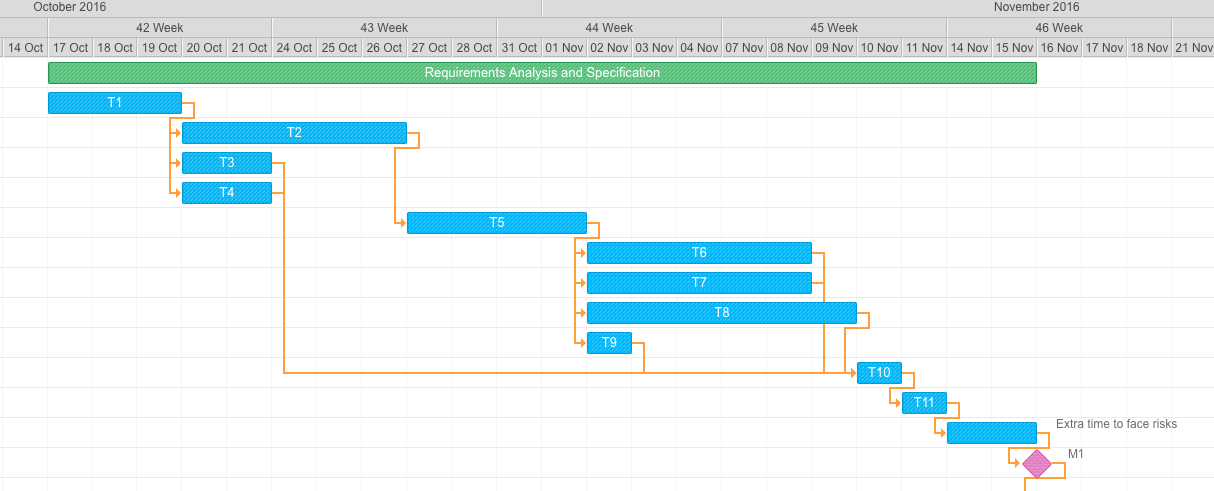
\includegraphics[scale=0.4]{{Figures/Gantt1.png}}
    \label{fig:1FirstScreen}
    \caption{Gantt Diagram of Requirements Analysis and Specification}
\end{figure}

\begin{figure}[h!]
    \centering
    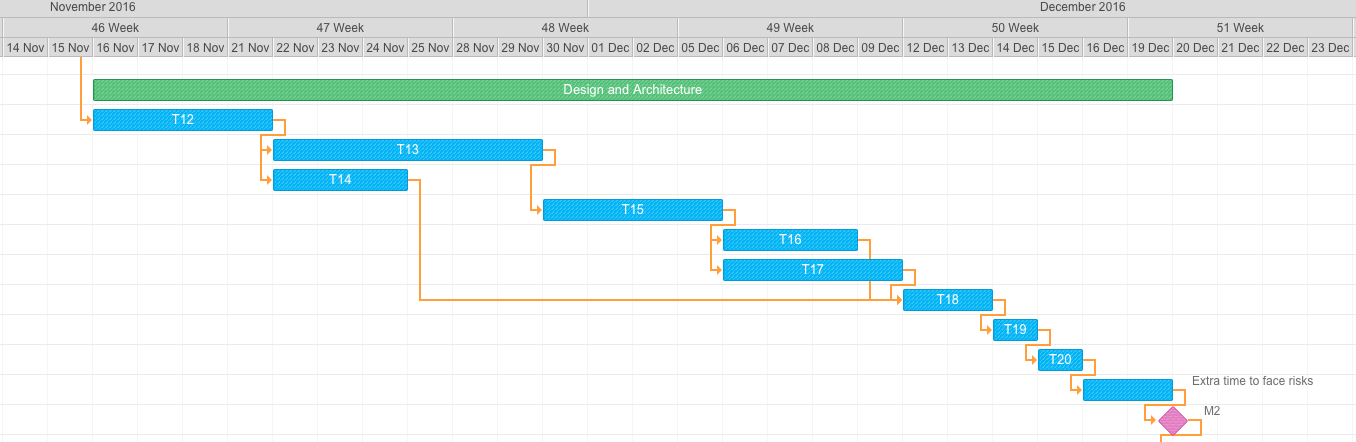
\includegraphics[scale=0.35]{{Figures/Gantt2.png}}
    \label{fig:1FirstScreen}
    \caption{Gantt Diagram of Design and Architecture}
\end{figure}

\begin{figure}[p!]
    \centering
    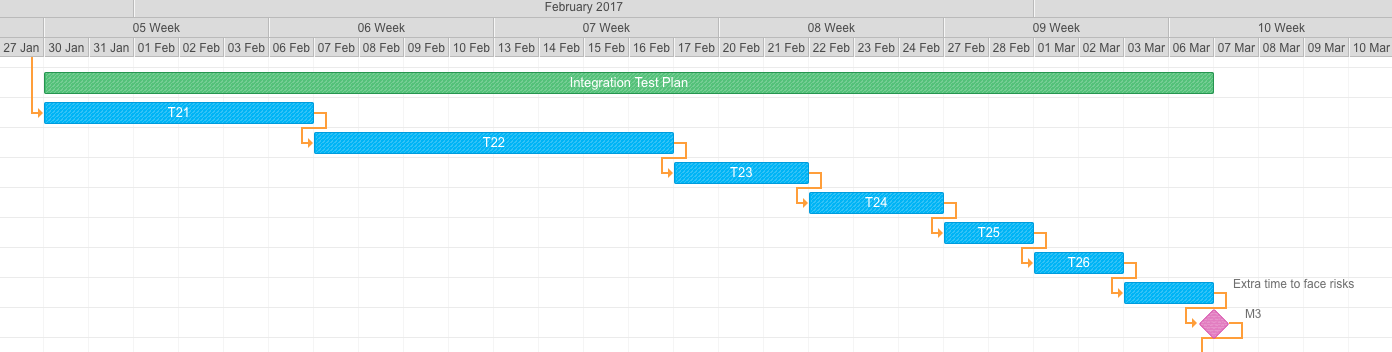
\includegraphics[scale=0.5]{{Figures/Gantt3.png}}
    \label{fig:1FirstScreen}
    \caption{Gantt Diagram of Integration Test Plan}
\end{figure}

\begin{figure}[p!]
    \centering
    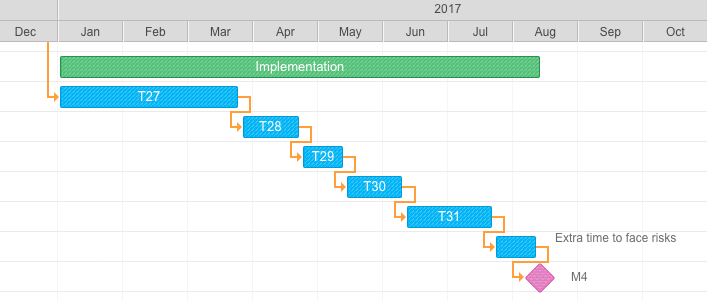
\includegraphics[scale=0.6]{{Figures/Gantt4.png}}
    \label{fig:1FirstScreen}
    \caption{Gantt Diagram of Implementation}
\end{figure}

\newpage
\subsection{Resource Allocation}
This section contains a table for each phase of the project where each of the previous tasks is assigned to at least one member of the group.\\

\noindent
\begin{tabular}{| l | c | c | c | c | c | c | c | c | c | c | c |}
\hline
\textbf{Member} & \textbf{T1} & \textbf{T2} & \textbf{T3} & \textbf{T4} & \textbf{T5} & \textbf{T6} & \textbf{T7} & \textbf{T8} & \textbf{T9} & \textbf{T10} & \textbf{T11}\\
\hline
Piccirillo Luca &  &  &  &  &  &  &  &  &  &  & \\
\hline
Zampogna Gian Luca &  &  &  &  &  &  &  &  &  &  & \\
\hline
Zini Edoardo &  &  &  &  &  &  &  &  &  &  & \\
\hline
\end{tabular}

\bigskip

\noindent
\begin{tabular}{| l | c | c | c | c | c | c | c | c | c |}
\hline
\textbf{Member} & \textbf{T12} & \textbf{T13} & \textbf{T14} & \textbf{T15} & \textbf{T16} & \textbf{T17} & \textbf{T18} & \textbf{T19} & \textbf{T20}\\
\hline
Piccirillo Luca &  &  &  &  &  &  &  &  & \\
\hline
Zampogna Gian Luca &  &  &  &  &  &  &  &  & \\
\hline
Zini Edoardo &  &  &  &  &  &  &  &  & \\
\hline
\end{tabular}

\bigskip

\noindent
\begin{tabular}{| l | c | c | c | c | c | c |}
\hline
\textbf{Member} & \textbf{T21} & \textbf{T22} & \textbf{T23} & \textbf{T24} & \textbf{T25} & \textbf{T26}\\
\hline
Piccirillo Luca &  &  &  &  &  & \\
\hline
Zampogna Gian Luca &  &  &  &  &  & \\
\hline
Zini Edoardo &  &  &  &  &  & \\
\hline
\end{tabular}

\bigskip

\noindent
\begin{tabular}{| l | c | c | c | c | c |}
\hline
\textbf{Person} & \textbf{T27} & \textbf{T28} & \textbf{T29} & \textbf{T30} & \textbf{T31}\\
\hline
Piccirillo Luca &  &  &  &  &  \\
\hline
Zampogna Gian Luca &  &  &  &  &  \\
\hline
Zini Edoardo &  &  &  &  &  \\
\hline
\end{tabular}